\documentclass[11pt]{article}

\usepackage[
backend=biber,
style=apa,
citestyle=numeric-comp
]{biblatex}
\usepackage{graphicx}
\usepackage{subcaption}
\usepackage[capitalise]{cleveref}
\newcommand{\twocolfigwidth}{0.49\textwidth}
\newcommand{\capshift}{-6mm}
\usepackage[font=small,labelfont=bf]{caption}


\title{Reproducing Resampling Paper Figure 1a}

\author{Iman Tabrizian}

\addbibresource{fedlearning.bib}
\begin{document}

\maketitle

\section{Results}

In this section we present the results for training a CNN on MNIST.
\cref{fig:mnist} shows that Krum\cite{krum} performs worse than
FedAvg~\cite{fedavg} when being trained on non-i.i.d.  dataset.
\cref{fig:krum-select} shows that Krum favors certain clients more and some of
the clients are almost never selected.  The reason is that Krum has been
designed for detecting byzantine workers in i.i.d.\ setting.

\cref{fig:krum-dir} shows the gradient selected by Krum when the number of
byzantine workers is equal to 1 and 0. When the number of byzantine workers is 0
Krum chooses the gradient closest to the majority of gradients. In our very
special case $n-f-2=1$ (\cref{fig:krum-dir} left), Krum chooses the gradient
with closest distance to another gradient. In this special case, the selected
gradient is not unique. We only show one of the possible gradients.

It is important to note here that the optimization employed here does not use
any momentum or weight decaying algorithm. 

\begin{figure}[ht]
    \begin{subfigure}[b]{\twocolfigwidth}
        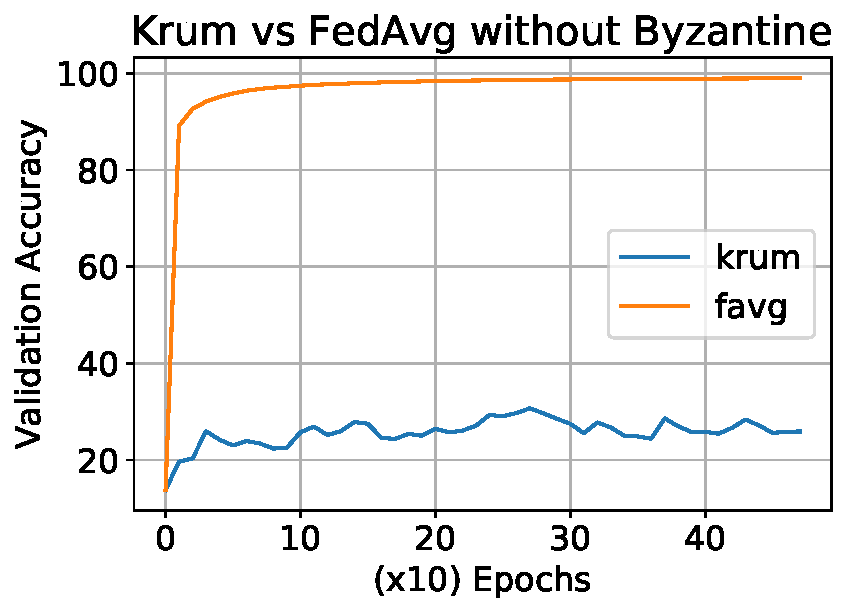
\includegraphics[width=\textwidth]{figs/krum-vacc}
        \caption{Validation Accuracy}
    \end{subfigure}
    \begin{subfigure}[b]{\twocolfigwidth}
        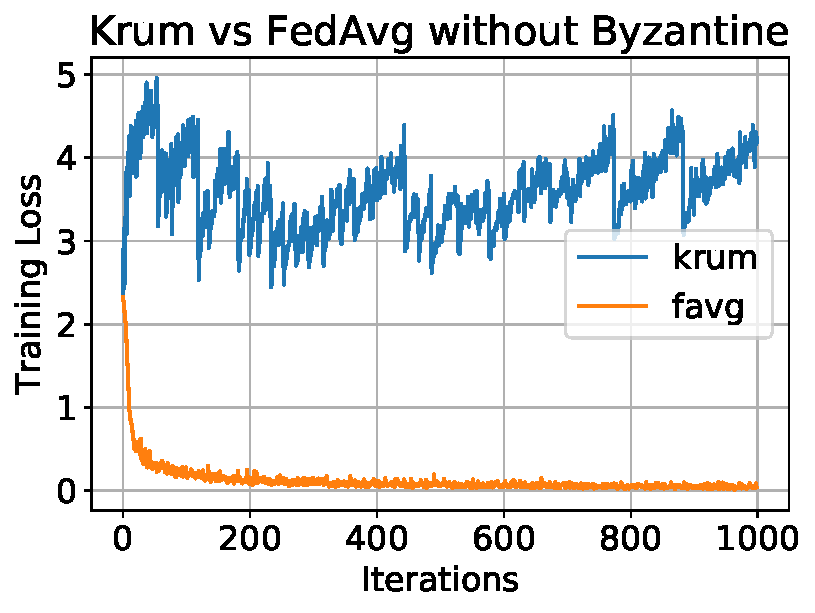
\includegraphics[width=\textwidth]{figs/krum-loss}
        \caption{Training Loss}
    \end{subfigure}
    \centering
    \caption{Training on Heterogeneous MNIST}
    \label{fig:mnist}
\end{figure}

\begin{figure}[ht]
    \begin{subfigure}[b]{\twocolfigwidth}
        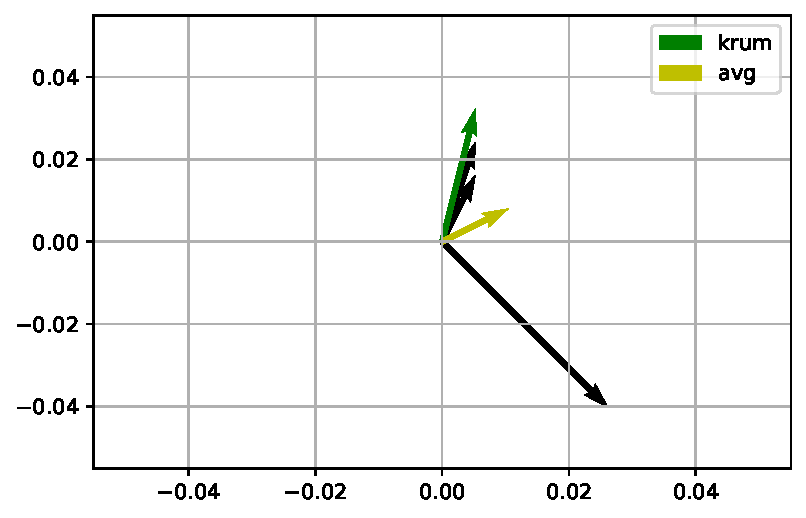
\includegraphics[width=\textwidth]{figs/krum-single}
        \caption{$f=1$, the vector that is closest to one other
        vector is selected.}
    \end{subfigure}
    \begin{subfigure}[b]{\twocolfigwidth}
        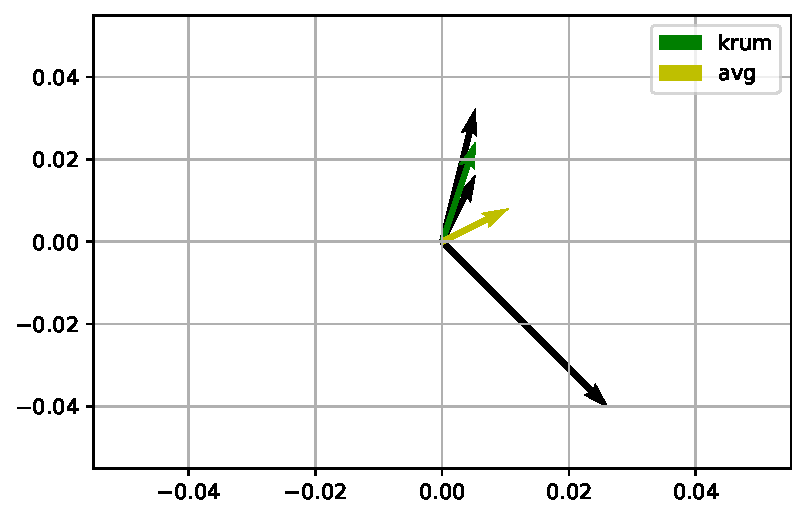
\includegraphics[width=\textwidth]{figs/krum-wadv}
        \caption{$f=0$, the vector that is closest to two other
        vectors is selected.}
    \end{subfigure}
    \centering
    \caption{Krum Direction, green vector is the vector selected by Krum. Black
    vectors are some hypothetical vectors}
    \label{fig:krum-dir}

\end{figure}

\begin{figure}[ht]
    \centering
    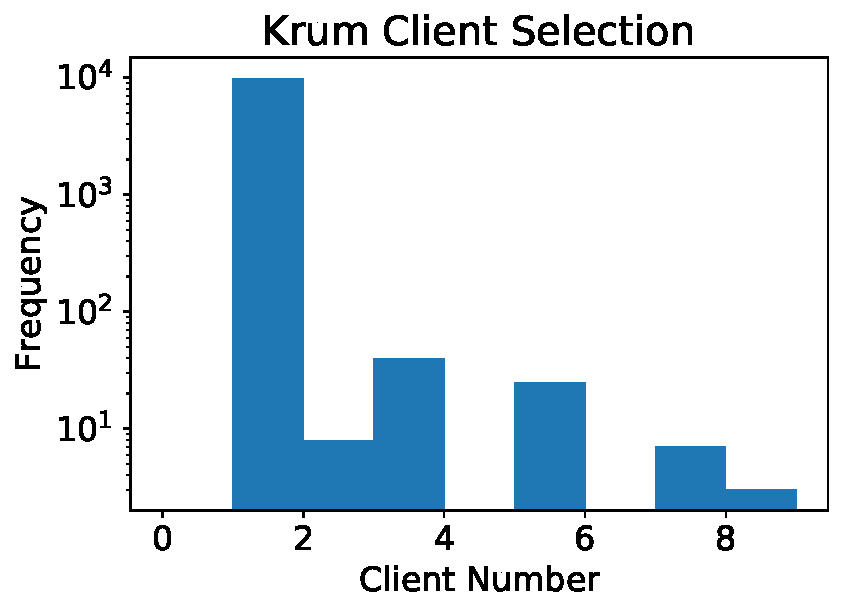
\includegraphics[width=0.5\textwidth]{figs/krum-selection}
    \caption{Krum Client Selection}
    \label{fig:krum-select}
\end{figure}
\printbibliography
\end{document}
